%%%%%%%%%%%%%%%%%%%%%%%%%%%%%%%%%%%%%%%%%%%%%%%%%%%%
%%%             Metadata                         %%%
%%%%%%%%%%%%%%%%%%%%%%%%%%%%%%%%%%%%%%%%%%%%%%%%%%%%      


\title{Grundkurs Linguistik}

\subtitle{Semantik}

\author[aMyP]{
	{\small Antonio Machicao y Priemer}
%	\\
%	{\footnotesize \url{http://www.linguistik.hu-berlin.de/staff/amyp}\\
%	\href{mailto:mapriema@hu-berlin.de}{mapriema@hu-berlin.de}}
}

\institute{Institut für deutsche Sprache und Linguistik}

%%%%%%%%%%%%%%%%%%%%%%%%%      
\date{ }
%\publishers{\textbf{6. linguistischer Methodenworkshop \\ Humboldt-Universität zu Berlin}}

%\hyphenation{nobreak}


%%%%%%%%%%%%%%%%%%%%%%%%%%%%%%%%%%%%%%%%%%%%%%%%%%%%
%%%             Preamble's End                   %%%
%%%%%%%%%%%%%%%%%%%%%%%%%%%%%%%%%%%%%%%%%%%%%%%%%%%%      


%%%%%%%%%%%%%%%%%%%%%%%%%      
\huberlintitlepage

\iftoggle{toc}{
\frame{
\begin{multicols}{2}
	\frametitle{Inhaltsverzeichnis}\tableofcontents
	%[pausesections]
\end{multicols}
}
}
%%%%%%%%%%%%%%%%%%%%%%%%%%%%%%%%%%%
%%%%%%%%%%%%%%%%%%%%%%%%%%%%%%%%%%

%%\nocite{Brandt&Co06a} \nocite{Glueck05a} \nocite{Grewendorf&Co91a} 
\nocite{Luedeling2009} \nocite{Meibauer&Co07a} %\nocite{MuellerS15b}
\nocite{Repp&Co15a}

%%%%%%%%%%%%%%%%%%%%%%%%%%%%%%%%%%%
%%%%%%%%%%%%%%%%%%%%%%%%%%%%%%%%%%
\begin{frame}
\frametitle{Begleitlektüre}

\begin{itemize}
	\item AM S.~95--106
	\item \citet{Lohnstein11}: Kapitel 4 (S.~34--49)
\end{itemize}
\end{frame}


%%%%%%%%%%%%%%%%%%%%%%%%%%%%%%%%%%%
%%%%%%%%%%%%%%%%%%%%%%%%%%%%%%%%%%%
%
\section{Einführung}
%
%\frame{
%\begin{multicols}{2}
%\frametitle{~}
%	\tableofcontents[currentsection]
%\end{multicols}
%}
%%%%%%%%%%%%%%%%%%%%%%%%%%%%%%%%%%%%%

\begin{frame}
\frametitle{Einführung}

\begin{itemize}
	\item Semantik (Bedeutungslehre)
	\item []
	\item Teildisziplin der \textbf{Linguistik} \ras \textbf{Bedeutung} von einfachen und zusammengesetzten \textbf{natürlichsprachlichen Ausdrücken}
	\item []
	\item Durch morphologische und syntaktische Kompetenz \ras Produktion von unendlich vielen Wörtern und Sätzen
	\item[]
	\item Aufgabe der Semantik \ras Welche Kenntnisse besitzen wir, um diese unendlich vielen sprachlichen (einfachen oder komplexen) Ausdrücke zu verstehen (oder zu produzieren) \ras Wie muss unsere \textbf{semantische Kompetenz} aussehen, welche sind die \textbf{zugrunde liegenden Fähigkeiten}?
\end{itemize}


\end{frame}


%%%%%%%%%%%%%%%%%%%%%%%%%%%%%%%%%%%%%%%%

\begin{frame}
\frametitle{Einführung}

\begin{itemize}
	\item Gegenstandsbereiche anderer Teilbereiche der Linguistik:
		
		\begin{itemize}
			\item Phonologie, die Morphologie und die Syntax \ras leichter erfassbar (Datensammlungen, wie Korpora oder in Tonaufnahmen)
		\end{itemize}
	
	\item []	
	\item Bedeutung lässt sich schwer messen oder erfassen
		
		\begin{itemize}
			\item Methoden: muttersprachliche Intuition, psycholinguistische Experimente
		\end{itemize}
		
	\item[]	
	\item Teildisziplin der \textbf{Semiotik} (Zeichenlehre) \ras Bedeutung von \textbf{Zeichen im Allgemeinen} (s. Symbol, Ikone, Index) und \textbf{Beziehung} zwischen Zeichen und seiner Bedeutung
\end{itemize}

\end{frame}


%%%%%%%%%%%%%%%%%%%%%%%%%%%%%%%%%%%%%
%
\section{Zeichen}
%
\iftoggle{toc}{
\frame{
\begin{multicols}{2}
\frametitle{~}
	\tableofcontents[currentsection]
\end{multicols}
}
}
%%%%%%%%%%%%%%%%%%%%%%%%%%%%%%%%%%%%%%%%
\begin{frame}
\frametitle{Zeichen}

\begin{itemize}
	\item Zeichen bestehen aus zwei Komponenten:
		
		\begin{itemize}
			\item \textbf{Inhaltsseite}
			\item \textbf{Ausdrucksseite}
		\end{itemize}
		
	\item Untersuchung der Beziehung zwischen Inhalts- und Ausdrucksseite u.\,a. durch Ferdinand de Saussure und Karl Bühler (Organonmodell) zu Beginn des XX. Jh.
	\item De Saussure: Ein linguistisches Zeichen ist nicht eine Verbindung zwischen einem Ding und einem Namen, sondern zwischen einem \textbf{Konzept} (frz. signifié/ dt. Signifikat) und einem \textbf{Lautmuster} (frz. signifiant/ dt. Signifikant).
	\item Bilaterale Zeichenkonzeption von de Saussure wurde ergänzt
		
		\begin{itemize}
			\item Mit sprachlichen Zeichen beziehen wir uns nicht auf Begriffen, sondern auf \textbf{Referenten} auf der Welt, auf \gqq{Gegenstände}.
		\end{itemize}
		
\end{itemize}

\end{frame}


%%%%%%%%%%%%%%%%%%%%%%%%%%%%%%%%%%%

\begin{frame}
\frametitle{Zeichen}

\begin{figure}
\centering
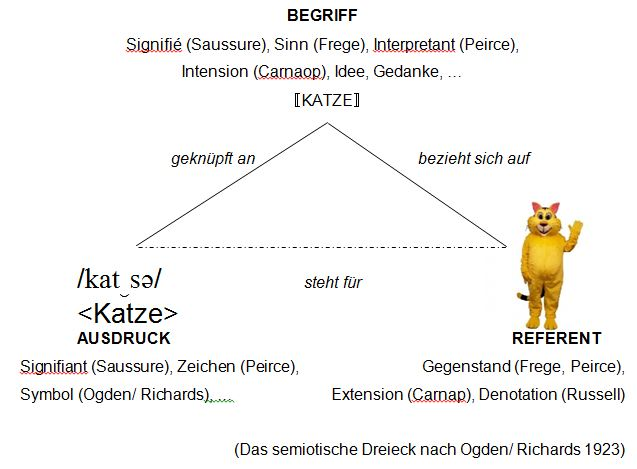
\includegraphics[scale=0.5]{material/07SemiotischesDreieck}
\end{figure}

\end{frame}


%%%%%%%%%%%%%%%%%%%%%%%%%%%%%%%%%

\begin{frame}
\frametitle{Zeichen}

\begin{itemize}
	\item Sprachliches Zeichen (Ausdruck) hat \textbf{keinen direkten Bezug} auf einen Referenten
	\item []	
	\item Bezug zwischen Ausdruck und Referent \textbf{durch den Begriff} (in der aktuellen sprachlichen Welt)

	\begin{itemize}
		\item \textbf{Ausdruck} ist an einen \textbf{Begriff}/ Konzept gekoppelt, der schließlich die \textbf{Referenz} ermöglicht
	\end{itemize}
	
\end{itemize}
	
\end{frame}


%%%%%%%%%%%%%%%%%%%%%%%%%%%%%%%%%%%

\begin{frame}
\frametitle{Zeichen}

\begin{itemize}
	\item Wichtige Eigenschaften von Zeichen (de Saussure):
	
	\begin{itemize}
		\item Verbindung zwischen Zeichenform und Zeicheninhalt $\rightarrow$ \textbf{arbiträr}
		
		\begin{itemize}
			\item Derselbe Inhalt aber in unterschiedlichen Sprachen durch verschiedene (lautliche) Formen
			\item \gq{KATZE}: Dt.: Katze, Sp.: gato, Frz.: chat
			\item Von der Form eines sprachlichen Zeichens kann man nicht auf seinen Inhalt/ Referenten schließen (Ausnahme: Onomatopoesie).
		\end{itemize}
		
		\item []		
		\item Verbindung zwischen Zeichenform und Zeicheninhalt \ras \textbf{konventionell}
		
		\begin{itemize}
			\item Es muss in einer Sprachgemeinschaft \textbf{festgelegt} sein, welche Form mit welchem Inhalt verknüpft ist. Dies muss so \textbf{gelernt} werden und kann \textbf{nicht beliebig verändert} werden.
		\end{itemize}
		
	\end{itemize}
	
\end{itemize}

\end{frame}


%%%%%%%%%%%%%%%%%%%%%%%%%%%%%%%

\begin{frame}
\frametitle{Zeichen}

\begin{itemize}
	\item Bsp. Gebärdensprachen:
	
	\begin{itemize}
		\item \textbf{Konventionalität} als grundlegendere Eigenschaft
		\item[]
		\item Viele verwendete Zeichen in Gebärdensprachen haben ikonische oder semi-ikonische Eigenschaften.\\
\ras Verbindung zwischen einer Gebärde und ihrem Inhalt nicht (immer) völlig arbiträr!
		\item[]		
		\item Eine Gebärde kann aber nicht einfach durch eine andere ersetzt werden \ras Konventionalität
		\item[]
		\item Der ikonische (oder semi-ikonische) Charakter von Gebärden geht mit der Zeit auch verloren, und somit werden diese Zeichen auch \textbf{arbiträr}.
	\end{itemize}
	
\end{itemize}

\end{frame}


%%%%%%%%%%%%%%%%%%%%%%%%%%%%%%%%%%%
%
\section{Bedeutung}
%
\iftoggle{toc}{
\frame{
\begin{multicols}{2}
\frametitle{~}
	\tableofcontents[currentsection]
\end{multicols}
}
}
%%%%%%%%%%%%%%%%%%%%%%%%%%%%%%%%%%%%%%

\begin{frame}
\frametitle{Bedeutung}

\begin{itemize}
	\item Bedeutungsbegriff \ras vielschichtig
	\item[]
	\item Bedeutung ist Untersuchungsgegenstand der
	
	\begin{itemize}
		\item Semantik\\ \&
		\item Pragmatik\\ 
		\vspace{3mm}
		Keine klare Trennung!
	\end{itemize}
	
	\item Semantik \ras kontextunabhängige Bedeutungsaspekte
	\item[]
	\item Pragmatik \ras kontextabhängige Bedeutungsaspekte
\end{itemize}

\end{frame}


%%%%%%%%%%%%%%%%%%%%%%%%%%%%%%%%%%%

\begin{frame}
\frametitle{Bedeutung}

\begin{itemize}
	\item Drei Ebenen der Bedeutung:
	
	\begin{itemize}
		\item Ausdrucksbedeutung (auch Satzbedeutung)
		\item Äußerungsbedeutung
		\item Sprecherbedeutung (Kommunikativer Sinn)
	\end{itemize}
	
	\item[]
	\item Ausdrucksbedeutung (Satzbedeutung)
	
	\begin{itemize}
		\item Die wörtliche Bedeutung, die sich systematisch aus der Bedeutung der Elementen und der Art der Verknüpfung ableiten lässt.
		\item Unabhängig vom Äußerungskontext
	\end{itemize}

\end{itemize}

\end{frame}


%%%%%%%%%%%%%%%%%%%%%%%%%%%%%%%%%%%

\begin{frame}
\frametitle{Bedeutung}

\begin{itemize}
	\item Ausdrucksbedeutung (Satzbedeutung)
	
	\ea \label{ex1}Peter hat das ganze Brot aufgegessen.
	\z
	
	\begin{itemize}
		\item Der Satz in \ref{ex1} hat demnach in etwa die Satzbedeutung:\\
		\vspace{5mm}
		Es gibt ein Individuum, das \textbf{Peter} genannt wird,
und für dieses Individuum trifft die Eigenschaft zu (\textbf{Deklarativsatz}),
\textbf{das Brot gänzlich} aufgegessen zu haben (\textbf{Vergangenheitsform}).
	\end{itemize}
	
\end{itemize}

\end{frame}


%%%%%%%%%%%%%%%%%%%%%%%%%%%%%%%%%%%

\begin{frame}
\frametitle{Bedeutung}

\begin{itemize}
	\item Äußerungsbedeutung
	
	\begin{itemize}
		\item Sie bezieht sich jedoch auf die in einem bestimmten, situativen Kontext weiter spezifizierte Bedeutung eines Ausdrucks.
		\item[]
		\item Wenn Peter an seinem 20. Geburtstag am 20. Oktober 2010 um 10 Uhr morgens das Brot aufgegessen hat, ist die Äußerung des Satzes um 11 Uhr morgens desselben Tages immer noch wahr.
		\item[]
		\item In diesem Fall redet man auch vom Äußerungskontext, der notwendig ist, um den Satz zu disambiguieren und seine Referenz zu bestimmen (s. deiktische Ausdrücke).
	\end{itemize}
	
\end{itemize}

\end{frame}


%%%%%%%%%%%%%%%%%%%%%%%%%%%%%%%%%%%

\begin{frame}
\frametitle{Bedeutung}

\begin{itemize}
	\item Sprecherbedeutung (oder kommunikativer Sinn)
	
	\begin{itemize}
		\item Sie meint hingegen die Sprecherintention
		\item[]
		\item Was meint der Sprecher eigentlich mit der Äußerung des Satzes?
		\item[]
		\item Sprecher von Satz \ref{ex1} kann z.B.:
		
		\begin{itemize}
			\item jemanden auffordern, Brot für das Frühstück zu kaufen, weil Peter alles aufgegessen hat.
		\end{itemize}
		
		\item In einigen Äußerungskontexten kann die Satzbedeutung eines Ausdrucks stark von seiner Sprecherbedeutung abweichen.
	\end{itemize}

\end{itemize}

\end{frame}


%%%%%%%%%%%%%%%%%%%%%%%%%%%%%%%%%%%

\begin{frame}
\frametitle{Bedeutung}

\begin{itemize}
	\item Sprecherbedeutung (oder kommunikativer Sinn)
	
	\begin{itemize}
		\item Beispiel \ref{ex2}: Aufforderung, den Raum zu verlassen
		\item[]
		\item Beispiel \ref{ex3}: ironischer Kommentar zu jemandem, der etwas falsch gemacht hat.\\
		
		\ea \label{ex2} Da ist die Tür!
		\z
		
		\ea \label{ex3}Das hast du aber toll gemacht!
		\z
		
	\end{itemize}
	
\end{itemize}

\end{frame}


%%%%%%%%%%%%%%%%%%%%%%%%%%%%%%%%%%

\begin{frame}
\frametitle{Bedeutung}

\begin{itemize}
	\item Satzbedeutung \ras Gegenstand der Semantik
	\item[]
	\item Sprecherbedeutung \ras Gegenstand der Pragmatik
	\item[]
	\item Äußerungsbedeutung \ras  sowohl in der Semantik (deiktische Elemente) als auch in der Pragmatik (Kontext) berücksichtigt
\end{itemize}

\end{frame}


%%%%%%%%%%%%%%%%%%%%%%%%%%%%%%%%%%%
%
\section{Lexikalische Semantik (Wortbedeutung)}
%
\iftoggle{toc}{
\frame{
\begin{multicols}{2}
\frametitle{~}
	\tableofcontents[currentsection]
\end{multicols}
}
}
%%%%%%%%%%%%%%%%%%%%%%%%%%%%%%%%%%%%%%%

\begin{frame}
\frametitle{Lexikalische Semantik (Wortbedeutung)}

\begin{itemize}
	\item Wortbedeutung \ras konventionalisierter und kontextunabhängiger Inhalt eines Ausdrucks
	\item[]
	\item Lexikalische Semantik:
	
	\begin{itemize}
		\item Erfassung des invariablen Inhalts eines Wortes
		\item Repräsentation und Organisation des Inhalts
	\end{itemize}
	
	\item[]
	\item Siehe: Merkmalshypothese, Prototypentheorie, Wortfeldrelationen, etc.
\end{itemize}


\end{frame}


%%%%%%%%%%%%%%%%%%%%%%%%%%%%%%%%%%%
%
\subsection{Sinnrelationen}
%
%\frame{
%\begin{multicols}{2}
%\frametitle{~}
%	\tableofcontents[currentsection]
%\end{multicols}
%}
%%%%%%%%%%%%%%%%%%%%%%%%%%%%%%%%%%%%%%%

\begin{frame}
\frametitle{Sinnrelationen}

\begin{itemize}
	\item Zusammenhang zwischen den Bedeutungen von Ausdrücken
	\item[]
	\item Systematisch erfassbare Relationen:
	
\vspace{5mm}
	
	\begin{itemize}
		\item Synonymie
		\item[]
		\item Hyponymie / Hyperonymie (Kohyponymie)
		\item[]		
		\item Meronymie
		\item[]
 		\item Antonymie
	\end{itemize}
	
\end{itemize}

\end{frame}


%%%%%%%%%%%%%%%%%%%%%%%%%%%%%%%%%%%

\begin{frame}
\frametitle{Sinnrelationen}

\begin{itemize}
	\item \textbf{Synonymie}\\Zwei Ausdrücke X und Y sind Synonyme, wenn der Austausch von X durch Y und umgekehrt in allen Kontexten bei Wahrung der Wahrheit (salva veritate) erfolgt.
	\item[]
	\item Bikonditional: $\leftrightarrow$
	
	\eal
		\ex Apfelsine $\leftrightarrow$ Orange
		\ex anfangen $\leftrightarrow$ beginnen
		\ex sterben $\leftrightarrow$ abkratzen
		\ex Treppe $\leftrightarrow$ Stiege
		\ex Brötchen $\leftrightarrow$ Schrippe $\leftrightarrow$ Semmel
	\zl
	
	\item Konnotative, regionale und registerabhängige Unterschiede
\end{itemize}

\end{frame}


%%%%%%%%%%%%%%%%%%%%%%%%%%%%%%%%%%%

\begin{frame}
\frametitle{Sinnrelationen}

\begin{itemize}
	\item \textbf{Hyperonymie / Hyponymie}\\
Ein Ausdruck X ist ein Hyperonym von Y, wenn die Bedeutung von Y in der Bedeutung von X enthalten ist.
Ein Ausdruck Y ist ein Hyponym von X, wenn die Bedeutung von Y in der Bedeutung von X enthalten ist.
	\item[]	
	\item Transitive Relation
	\item[]
	\item Implikation: \ras
	
	\begin{itemize}
		\item Y ist ein X
		
		\eal 
		\ex Küchenstuhl \ras Stuhl \ras Sitzgelegenheit
		\ex erschie\ss{}en \ras töten
		\zl
		
	\end{itemize}
	
\end{itemize}

\end{frame}


%%%%%%%%%%%%%%%%%%%%%%%%%%%%%%%%%%%

\begin{frame}
\frametitle{Sinnrelationen}

\begin{itemize}
	\item \textbf{Kohyponymie}\\
Ein Ausdruck X ist ein Kohyponym von Z (und umgekehrt), wenn die Bedeutung von X und Z in der Bedeutung von Y enthalten ist. Kohyponyme schließen einander aus (Inkompatibilität)

\eal
\ex Drehstuhl $|$ Küchenstuhl \ras Stuhl \ras Sitzgelegenheit
\ex erschießen / erwürgen / erdrosseln \ras töten
\zl


	\item[]
	\item Hyperonymie $|$ Hyponymie: Basis für Taxonomien

\end{itemize}

\end{frame}


%%%%%%%%%%%%%%%%%%%%%%%%%%%%%%%%%%

\begin{frame}
\frametitle{Sinnrelationen}

\begin{itemize}
	\item \textbf{Meronymie}\\
Ein Ausdruck X ist ein Meronym von Y, wenn X ein Teil von Y ist.

\vspace{5mm}
	
	\eal
	\ex Finger > Hand > Arm > Oberkörper > Körper
	\ex Rad > Auto
	\zl
	
	\item[]
	\item Transitiv: 
		
	\ea die Manschette des Ärmels, der Ärmel der Jacke \ras die Manschette der Jacke
	\z
		
	\item Intransitiv: 
		
	\ea der Griff der Tür, die Tür des Hauses \ras \# der Griff des Hauses
	\z
		
\end{itemize}

\end{frame}


%%%%%%%%%%%%%%%%%%%%%%%%%%%%%%%%%%%

\begin{frame}
\frametitle{Sinnrelationen}

\begin{itemize}
	\item \textbf{Antonymie}\\
          Ein Ausdruck X ist ein Antonym von Y,\\
          wenn X in irgendeinem Sinne das Gegenteil von Y ist.
	\item[]	
	\item X \ras $\lnot$ Y
	
	\eal 
		\ex fleißig -- faul
		\ex klug -- dumm
	\zl
	
\end{itemize}

\end{frame}


%%%%%%%%%%%%%%%%%%%%%%%%%%%%%%%%%%%

\begin{frame}
\frametitle{Sinnrelationen}

\begin{itemize}
	\item \textbf{Kontradiktorische Antonymie}\\
Ein Ausdruck X ist ein kontradiktorisches Antonym von Y, wenn die Negation von X die Bedeutung von Y ergibt und umgekehrt. (Eine drittes Z ist ausgeschlossen)
	\item Komplementarität: (X \ras $\lnot$ Y) \& ($\lnot$ X  \ras Y)
	\item Binär
	\item Beide Aussagen können nicht gleichzeitig wahr sein und auch nicht gleichzeitig falsch sein.
	
	\eal
		\ex krank -- gesund
		\ex lebendig -- tot
		\ex anwesend -- abwesend
	\zl
	
\end{itemize}

\end{frame}


%%%%%%%%%%%%%%%%%%%%%%%%%%%%%%%%%%%

\begin{frame}
\frametitle{Sinnrelationen}

\begin{itemize}
	\item \textbf{Konträre Antonymie}\\
Ein Ausdruck X ist ein konträres Antonym von Y, wenn X und Y nicht zugleich wahr sein können, aber beide können zugleich nicht zutreffen.
	\item[]
	\item Skalar: Antonymie mit Zwischenstufen
	\item[]
	\item Beide Aussagen können nicht gleichzeitig wahr sein, aber sie können gleichzeitig falsch sein.
	\item[]
	\item (X $\rightarrow \lnot$ Y) \& (Y $\rightarrow \lnot$ X)
	
	\eal
		\ex reich -- arm
		\ex kalt -- (kühl -- lau -- warm) -- heiß
	\zl
	
\end{itemize}

\end{frame}


%%%%%%%%%%%%%%%%%%%%%%%%%%%%%%%%%%%

\begin{frame}
\frametitle{Sinnrelationen}

\begin{itemize}
	\item \textbf{Ambiguität (Lexikalische Mehrdeutigkeit)}

\vspace{1em}

	\begin{itemize}
		\item \textbf{Homonymie}\\
Ein Ausdruck X und ein Ausdruck Y sind gleich in deren Form (phonetische oder graphische) aber unterschiedlich in deren Bedeutung, wobei X und Y unterschiedliche Ursprünge haben.
	\end{itemize}
\end{itemize}

\end{frame}


%%%%%%%%%%%%%%%%%%%%%%%%%%%%%%%%%%%

\begin{frame}
\frametitle{Sinnrelationen}

\begin{itemize}
	\item \textbf{Ambiguität (Lexikalische Mehrdeutigkeit)}

\vspace{1em}

	\begin{itemize}
		\item \textbf{Homonymie:}
		
		\begin{itemize}
			\item Homophonie:
			
			\eal
			\ex mahlen vs. malen 
			\ex sieben (7) vs. sieben
			\ex laut vs. laut (Präp.)
			\zl
			
			\item Homographie:
					
			\eal 
			\ex 'modern vs. mo'dern
			\ex Die Therapie des gebrochenen Beines beinhaltet das Fixieren in einer Beinhalterung.
			\zl
			
		\end{itemize}
		
	\end{itemize}
\end{itemize}

\end{frame}


%%%%%%%%%%%%%%%%%%%%%%%%%%%%%%%%%%%

\begin{frame}
\frametitle{Sinnrelationen}

\begin{itemize}
	\item \textbf{Ambiguität (Lexikalische Mehrdeutigkeit)}
	
\vspace{1em}

	\begin{itemize}
		\item \textbf{Polysemie}\\
Ein Ausdruck X und ein Ausdruck Y sind gleich in deren Form (phonetische und graphische) können aber unterschiedliche Bedeutungsvarianten voneinander sein. X und Y stehen in einem etymologischen Zusammenhang zueinander.

		\ea Schule, Oper, Grammatik
		\z

	\end{itemize}
	
\end{itemize}

\end{frame}


%%%%%%%%%%%%%%%%%%%%%%%%%%%%%%%%%%%
\iftoggle{uebung}{

\begin{frame}
\frametitle{Sinnrelationen}

\begin{itemize}
	\item \textbf{Übung:}
	
	\eal
	\ex Ballkleid -- Kleid
	\ex Bank -- Bank
	\ex Schraubenzieher -- Zange
	\ex gro\ss{} -- klein
	\ex Henkel -- Tasse
	\ex Ahorn -- Baum
	\ex essen -- verzehren
	\ex gerade -- ungerade
	\zl
		
\end{itemize}

\end{frame}

}
%%%%%%%%%%%%%%%%%%%%%%%%%%%%%%%%%%%%%%%%%
\iftoggle{ha-loesung}{

\begin{frame}
\frametitle{Lösung}
	
	\eal
	\ex Ballkleid -- Kleid: Hyponym/ Hyperonym
	\ex Bank -- Bank: Homonymie (-graphie und -phonie)
	\ex Schraubenzieher -- Zange: Kohyponymie
	\ex gro\ss{} -- klein: Konträre Antonymie
	\ex Henkel -- Tasse: Meronymie
	\ex Ahorn -- Baum: Hyponym/ Hyperonym
	\ex essen -- verzehren: Synonymie
	\ex gerade -- ungerade: Kontradiktorische Antonymie
	\zl

\end{frame}
}
%%%%%%%%%%%%%%%%%%%%%%%%%%%%%%%%%%%%%%%%%%%
%
\section{Satzsemantik (Satzbedeutung)}
%
\iftoggle{toc}{
\frame{
\begin{multicols}{2}
\frametitle{~}
	\tableofcontents[currentsection]
\end{multicols}
}
}
%%%%%%%%%%%%%%%%%%%%%%%%%%%%%%%%%%%%%%%%%%

\begin{frame}
\frametitle{Satzsemantik (Satzbedeutung)}

\begin{itemize}
	\item Wahrheitsbedingungen (Wittgenstein 1921)
	\item[]
	\item Die Bedeutung eines Satzes zu kennen, heißt, notwendige und hinreichende Bedingungen für die Wahrheit bzw. Falschheit des Satzes (= seine Wahrheitsbedingungen) zu kennen.
	\item[]
	\item Bedingungen in der aktuellen Welt (verschiedene Welten)
	
	
		\ea Martin kauft Brötchen.
		\z
		
	\begin{itemize}	
		\item Wahr oder Falsch (1 oder 0) \ras abhängig von der Welt
	\end{itemize}
	
\end{itemize}

\end{frame}


%%%%%%%%%%%%%%%%%%%%%%%%%%%%%%%%%%%%%%%%%%

\begin{frame}
\frametitle{Satzsemantik (Satzbedeutung)}

\begin{itemize}
	\item \textbf{Kompositionalitätsprinzip}\\
Die Bedeutung eines komplexen Ausdrucks ergibt sich aus der Bedeutung seiner unmittelbaren syntaktischen Teile und der Art und Weise, wie sie sich syntaktisch zusammensetzen.
	\item[]
	\item Auch Fregeprinzip genannt
\end{itemize}

\end{frame}


%%%%%%%%%%%%%%%%%%%%%%%%%%%%%%%%%%%%%%%%%%
%%%%%%%%%%%%%%%%%%%%%%%%%%%%%%%%%%%%%%%%%%
%
\subsection{Aussagenlogik}
%\frame{
%\begin{multicols}{2}
%\frametitle{~}
%	\tableofcontents[currentsection]
%\end{multicols}
%}
%%%%%%%%%%%%%%%%%%%%%%%%%%%%%%%%%%%%%%%%%%


\begin{frame}
\frametitle{Aussagenlogik}

\begin{itemize}
	\item Basierend auf dem Kompositionalitätsprinzip
	\item[]
	\item Teilgebiet der formalen Logik
	\item[]
	\item Verknüpfung von einfachen Aussagen
	\item[]
	\item Wie lässt sich der Wahrheitswert einer komplexen Aussage aus den Wahrheitswerten der in ihr enthaltenen einfachen Aussagen in Abhängigkeit der Verknüpfung errechnen?
\end{itemize}

\end{frame}


%%%%%%%%%%%%%%%%%%%%%%%%%%%%%%%%%%%%%%%%%%

\begin{frame}
\frametitle{Aussagenlogik}

\begin{itemize}
	\item Aussagen: p, q, r, s, \dots
	\item[]
	\item Konnektoren:
	
	\begin{itemize}
		\item Negation (NICHT): $\lnot$
		\item[]
		\item Konjunktion (UND): $\land$
		\item[]
		\item Disjunktion (UND/ODER): $\lor$
		\item[]
		\item Konditional (materiale Implikation) (WENN, DANN): \ras
		\item[]
		\item Bikonditional (GENAU DANN WENN): $\leftrightarrow$
	\end{itemize}
	
\end{itemize}

\end{frame}


%%%%%%%%%%%%%%%%%%%%%%%%%%%%%%%%%%%%%%%%%%

\begin{frame}
\frametitle{Aussagenlogik}

\begin{itemize}
	\item Negation (NICHT): $\lnot$
	
	\eal
		\ex p: Es regnet.
		\ex $\lnot$ p: Es regnet nicht.
	\zl
	
\end{itemize}

\begin{table}
\centering
\begin{tabular}{p{3cm}|p{3cm}}
\textbf{p} & \textbf{$\lnot$p}\\
\hline
1 & 0\\
\hline
0 & 1\\
\end{tabular}
\end{table}

\end{frame}


%%%%%%%%%%%%%%%%%%%%%%%%%%%%%%%%%%%%%%%%%%

\begin{frame}
\frametitle{Aussagenlogik}

\begin{itemize}
	\item Konjunktion (UND): $\land$
	
	\eal
		\ex p: Es regnet.
		\ex q: Es donnert.
		\ex p $\land$ q: Es regnet und es donnert.
	\zl

\end{itemize}
	

\begin{table}
\centering

\begin{tabular}{p{2cm}|p{2cm}|p{2cm}}
\textbf{p} & \textbf{q} & \textbf{p} $\land$ \textbf{q}\\
\hline
1 & 1 & 1\\
\hline
1 & 0 & 0\\
\hline
0 & 1 & 0\\
\hline 
0 & 0 & 0\\
\end{tabular}

\end{table}	

\end{frame}


%%%%%%%%%%%%%%%%%%%%%%%%%%%%%%%%%%%%%%%%%%

\begin{frame}
\frametitle{Aussagenlogik}

\begin{itemize}
	\item Disjunktion (UND/ODER): $\lor$

	\eal
		\ex p: Es regnet.
		\ex q: Es schneit.
		\ex p $\lor$ q : Es regnet oder es schneit.
	\zl

\end{itemize}


\begin{table}
\centering

\begin{tabular}{p{2cm}|p{2cm}|p{2cm}}
\textbf{p} & \textbf{q} & \textbf{p} $\lor$ \textbf{q}\\
\hline
1 & 1 & 1\\
\hline
1 & 0 & 1\\
\hline
0 & 1 & 1\\
\hline 
0 & 0 & 0\\
\end{tabular}

\end{table}		

\end{frame}


%%%%%%%%%%%%%%%%%%%%%%%%%%%%%%%%%%%

\begin{frame}
\frametitle{Aussagenlogik}

\begin{itemize}
	\item Konditional (materiale Implikation) (WENN, DANN): \ras
	
	\eal
		\ex p: Es regnet.
		\ex q: Die Stra\ss{}e ist nass.
		\ex p \ras q : Wenn es regnet, dann ist die Stra\ss{}e nass.
	\zl

\end{itemize}

\begin{table}
\centering
\begin{tabular}{p{2cm}|p{2cm}|p{2cm}}
\textbf{p} & \textbf{q} & \textbf{p} \ras \textbf{q}\\
\hline
1 & 1 & 1\\
\hline
1 & 0 & 0\\
\hline
0 & 1 & 1 (!)\\
\hline 
0 & 0 & 1\\
\end{tabular}
\end{table}	


\end{frame}


%%%%%%%%%%%%%%%%%%%%%%%%%%%%%%%%%%%

\begin{frame}
\frametitle{Aussagenlogik}

\begin{itemize}
	\item Bikonditional (GENAU DANN WENN): $\leftrightarrow$
	
	\eal
		\ex p: Peter raucht.
		\ex q: Maria trinkt.
		\ex p $\leftrightarrow$ q : Genau dann wenn Peter raucht, trinkt Maria.
	\zl

\end{itemize}


\begin{table}
\centering

\begin{tabular}{p{2cm}|p{2cm}|p{2cm}}
\textbf{p} & \textbf{q} & \textbf{p} $\leftrightarrow$ \textbf{q}\\
\hline
1 & 1 & 1\\
\hline
1 & 0 & 0\\
\hline
0 & 1 & 0\\
\hline 
0 & 0 & 1\\
\end{tabular}

\end{table}

\end{frame}


%%%%%%%%%%%%%%%%%%%%%%%%%%%%%%%%%%%
\iftoggle{uebung}{

\begin{frame}
\frametitle{Aussagenlogik}

\begin{itemize}
	\item Übungen:
	
	\vspace{1em}
	
	\begin{enumerate}
		\item Christiane schläft.
		\item []
		\item Norbert raucht nicht.
		\item[]
		\item Norbert raucht und Christiane schläft nicht.
		\item[]
		\item Wenn Norbert nicht raucht, schläft Christiane nicht.
		\item[]
		\item Wenn ich schlafe, träume ich.
		\item[]
		\item Ich schlafe nicht oder ich träume.
	\end{enumerate}
	
\end{itemize}

\end{frame}

%%%%%%%%%%%%%%%%%%%%%%%%%%%%%%%%%%%

%%%%%%%%%%%%%%%%%%%%%%%%%%%%%%%%%%%
\begin{frame}
\frametitle{Lösungen}

\begin{table}

\begin{minipage}{0.4\textwidth}
\centering
\begin{itemize}
\item[] \small{p: Christiane schläft.}
\end{itemize}
\scalebox{0.8}{
\begin{tabular}{l}
p\\
\hline
1\\
\hline
0\\
\end{tabular}
}
\end{minipage}
%	
\begin{minipage}{0.5\textwidth}
\centering
\begin{itemize}
\item[] \small{p: Norbert raucht.\\
q: Christiane schläft.}
\end{itemize}
\scalebox{0.8}{
\begin{tabular}{l|l|l}
p & q & p $\land \lnot $q\\
\hline
1 & 1 & 0\\
\hline
1 & 0 & 1\\
\hline
0 & 1 & 0 \\
\hline
0 & 0 & 0 \\
\end{tabular}
}
\end{minipage}

\vspace{1em}

\begin{minipage}{0.4\textwidth}
\centering
\begin{itemize}
\item[] \small{p: Norbert raucht.}
\end{itemize}
\scalebox{0.8}{
\begin{tabular}[b]{l|l}
p & $ \lnot $p \\
\hline
0 & 1 \\
\hline
1 & 0 \\
\end{tabular}}
\end{minipage}
%
\begin{minipage}{0.5\textwidth}
\centering
\begin{itemize}
\item[] \small{p: Norbert raucht.\\
q: Christiane schläft.}
\end{itemize}
\scalebox{0.8}{
\begin{tabular}{l|l|l}
p & q & $ \lnot $p \ras $ \lnot $q\\
\hline
1 & 1 & 0 \\
\hline
1 & 0 & 0 \\
\hline
0 & 1 & 0 \\
\hline
0 & 0 & 1 \\
\end{tabular}}
\end{minipage}
\end{table}

\end{frame}

%
%%%%%%%%%%%%%%%%%%%%%%%%%%%%%%%%%%%%

\begin{frame}
\frametitle{Lösungen}

\begin{table}

\begin{minipage}{0.48\textwidth}
\centering
\begin{itemize}
\item[] \small{p: Ich schlafe.\\
q: Ich träume.}
\end{itemize}
\scalebox{0.8}{
\begin{tabular}[b]{l|l|l}
p & q & p \ras q \\
\hline
1 & 1 & 1 \\
\hline
1 & 0 & 0 \\
\hline
0 & 1 & 1 \\
\hline
0 & 0 & 1 \\
\end{tabular}}
\end{minipage}
%
\begin{minipage}{0.48\textwidth}
\centering
\begin{itemize}
\item[] \small{p: Ich schlafe.\\
q: Ich träume.}
\end{itemize}
\scalebox{0.8}{
\begin{tabular}{l|l|l}
p & q & $\lnot$ p & $ \lnot $p \ras $ \lor $q\\
\hline
1 & 1 & 0 & 1 \\
\hline
1 & 0 & 0 & 0 \\
\hline
0 & 1 & 1 & 1 \\
\hline
0 & 0 & 1& 1 \\
\end{tabular}}
\end{minipage}
\end{table}

\end{frame}
}
%
%%%%%%%%%%%%%%%%%%%%%%%%%%%%%%%%%%%%

\begin{frame}
\frametitle{Aussagenlogik}

\begin{itemize}
	\item Übungen:

\vspace{1em}

	\begin{enumerate}
		\item Genau dann wenn ich Durst habe, trinke ich eine Cola.
		\item[]
		\item Es ist nicht der Fall, dass ich Durst habe, und es ist nicht der Fall, dass ich eine Cola trinke -- oder -- Es ist der Fall, dass ich Durst habe und es ist der Fall, dass ich eine Cola trinke.
		\item[]
		\item Es regnet oder, es scheint die Sonne und ich bin froh.
		\item[]
		\item Es regnet oder es scheint die Sonne, und es regnet oder ich bin froh.
		\item[]
		\item Es ist nicht der Fall, dass Norbert raucht oder Christiane schläft.
		\item[]
		\item Es ist nicht der Fall, dass Norbert raucht und es ist nicht der Fall dass Christiane schläft.
	\end{enumerate}
		
\end{itemize}


\end{frame}

%%%%%%%%%%%%%%%%%%%%%%%%%%%%%%%%%%%%%%%%%%%%%%%%%%%%%%%%%%%%%%%

%\iftoggle{loesung}{

\begin{frame}[shrink=20]
\frametitle{Lösungen}

\begin{table}

\begin{minipage}{0.4\textwidth}
\centering
\begin{itemize}
\item[] {\small p: Ich habe Durst.\\
q: Ich trinke eine Cola.}
\end{itemize}
\scalebox{0.8}{
\begin{tabular}{l|l|l}
p & q & p $ \leftrightarrow $ q\\
\hline
1 & 1 & 1\\
\hline
1 & 0 & 0\\
\hline
0 & 1 & 0\\
\hline
0 & 0 & 1\\
\end{tabular}
}
\end{minipage}
%	
\begin{minipage}{0.5\textwidth}
\centering
\begin{itemize}
\item[] {\small
p: Ich trinke Cola.\\
q: Ich habe Durst.}
\end{itemize}
\scalebox{0.80}{
\begin{tabular}{l|l|l|l|l}
p & q & $ \lnot $p $ \land \lnot $q & p $ \land $ q & ($ \lnot $p $ \land \lnot $q) $ \lor $ (p $ \land $ q)\\
\hline
1 & 1 & 0 & 1 & 1\\
\hline
1 & 0 & 0 & 0 & 0\\
\hline
0 & 1 & 0 & 0 & 0\\
\hline
0 & 0 & 1 & 0 & 1\\
\end{tabular}}
\end{minipage}

\vspace{1em}

\begin{minipage}{0.5\textwidth}
\centering
\begin{itemize}
\item[] {\small p: Es regnet.\\
q: Es scheint die Sonne.\\
s: Ich bin froh.}
\end{itemize}
\scalebox{0.8}{
\begin{tabular}{l|l|l|l|l}
p & q & s & q $\land $ s & p $\lor$ (q $\land $ s) \\
\hline
0 & 1 & 0 & 0 & 0\\
\hline
1 & 1 & 0 & 0 & 1\\
\hline
0 & 1 & 1 & 1 & 1\\
\hline
1 & 1 & 1 & 1 & 1\\
\hline
0 & 0 & 0 & 0 & 0\\
\hline
1 & 0 & 0 & 0 & 1\\
\hline
0 & 0 & 1 & 0 & 0\\
\hline
1 & 0 & 1 & 0 & 1\\
\end{tabular}
}
\end{minipage}
%
\begin{minipage}{0.4\textwidth}
\centering
\begin{itemize}
\item[] {\small p: Es regnet.\\
q: Es scheint die Sonne.\\
s: Ich bin froh.}
\end{itemize}
\scalebox{0.8}{
\begin{tabular}[b]{l|l|l|l|l|l}
p & q & s & p $ \lor $ q & p $ \lor $ s & (p $ \lor $ q) $ \land $ (p $ \lor $ s) \\
\hline
1 & 0 & 0 & 1 & 1 & 1\\
\hline
1 & 0 & 1 & 1 & 1 & 1\\
\hline
1 & 1 & 0 & 1 & 1 & 1\\
\hline
1 & 1 & 1 & 1 & 1 & 1\\
\hline
0 & 0 & 0 & 0 & 0 & 0\\
\hline
0 & 0 & 1 & 0 & 1 & 0\\
\hline
0 & 1 & 0 & 1 & 0 & 0\\
\hline
0 & 1 & 1 & 1 & 1 & 1\\

\end{tabular}}
\end{minipage}
\end{table}

\end{frame}

%%%%%%%%%%%%%%%%%%%%%%%%%
\begin{frame}
\frametitle{Lösungen}

\begin{table}

\begin{minipage}{0.48\textwidth}
\centering
\begin{itemize}
\item[] p: Norbert raucht.\\
q: Christiane schläft.
\end{itemize}
\scalebox{0.8}{
\begin{tabular}{l|l|l}
p & q & $ \lnot $ (p $ \lor $q)\\
\hline
1 & 1 & 0 \\
\hline
1 & 0 & 0 \\
\hline
0 & 1 & 0 \\
\hline
0 & 0 & 1 \\
\end{tabular}}
\end{minipage}
%
\begin{minipage}{0.48\textwidth}
\centering
\begin{itemize}
\item[] p: Norbert schläft.\\
q: Christine schläft.
\end{itemize}
\begin{tabular}{l|l|l}
p & q & $ \lnot $p $ \land $ $ \lnot $q\\
\hline
1 & 1 & 0\\
\hline
1 & 0 & 0\\
\hline
0 & 1 & 0\\
\hline
0 & 0 & 1\\
\end{tabular}
\end{minipage}

\end{table}
\end{frame}
%}
%%%%%%%%%%%%%%%%%%%%%%%%%%%%%%%%%%%

\begin{frame}
\frametitle{Aussagenlogik}
	
\begin{itemize}
	\item Übungen:

\vspace{1em}

	\begin{enumerate}
		\item Christiane schläft. (p)
		\item[]
		\item Norbert raucht nicht. ($\lnot$p)
		\item[]
		\item Norbert raucht und Christiane schläft nicht. (p $\land \lnot$ q)
		\item[]
		\item Wenn Norbert nicht raucht, schläft Christiane nicht. ($\lnot$ p \ras $\lnot$ q)
	\end{enumerate}

\item Konditional:

	\begin{enumerate}\setcounter{enumi}{4}
		\item Wenn ich schlafe, träume ich. ( p \ras q)
		\item[]
		\item Ich schlafe nicht oder ich träume. ($\lnot$ p $\lor$ q)
	\end{enumerate}
	
\end{itemize}

\end{frame}


%%%%%%%%%%%%%%%%%%%%%%%%%%%%%%%%%%%

\begin{frame}
\frametitle{Aussagenlogik}

\begin{itemize}
	\item Übungen: 
	
\vspace{1em}

	\begin{itemize}
		\item Bikonditional:
	
		\begin{enumerate}
			\item Genau dann wenn ich Durst habe, trinke ich eine Cola. (p $\leftrightarrow$ q)
			\item[]
			\item Es ist nicht der Fall, dass ich Durst habe, und es ist nicht der Fall, dass ich eine Cola trinke – oder – Es ist der Fall, dass ich Durst habe und es ist der Fall, dass ich eine Cola trinke. ($\lnot$ p $\leftrightarrow \lnot$ q) $\lor$ (p $\leftrightarrow$ q)
		\end{enumerate}
	
		\item Distributivität:
	
		\begin{enumerate}\setcounter{enumi}{2}
			\item Es regnet oder -- es scheint die Sonne und ich bin froh. (p  $\lor$ (q $\land$ r))
			\item[]
			\item Es regnet oder es scheint die Sonne, und es regnet oder ich bin froh. ((p $\lor$ q) $\land$ (p $\lor$ r))
		\end{enumerate}

	\end{itemize}

\end{itemize}



\end{frame}


%%%%%%%%%%%%%%%%%%%%%%%%%%%%%%%%%%%

\begin{frame}
\frametitle{Aussagenlogik}

\begin{itemize}
\item Übungen:

	\begin{itemize}
		\item De Morgans Gesetze:
	
		\begin{enumerate}
			\item Es ist nicht der Fall, dass Norbert raucht oder Christiane schläft. $\lnot$ (p $\lor$ q)
			\item[]
			\item Es ist nicht der Fall, dass Norbert raucht und es ist nicht der Fall dass Christiane schläft. ($\lnot$ p $\land \lnot$ q)
		\end{enumerate}
		
	\end{itemize}

\end{itemize}


\end{frame}


%%%%%%%%%%%%%%%%%%%%%%%%%%%%%%%%%%%

\begin{frame}
\frametitle{Aussagenlogik}

\begin{itemize}
	\item \textbf{Tautologie}
	
	\begin{itemize}
		\item Aussage, die stets wahr ist (unabhängig von den
Ausgangswerten der beteiligten Aussagen)
		
		\ea Es regnet oder es regnet nicht.
		\z
		
	\end{itemize}
	
	\item \textbf{Kontradiktion}
	
	\begin{itemize}
		\item  Aussage, die stets falsch ist (unabhängig von den
Ausgangswerten der beteiligten Aussagen)

		\ea Es regnet und es regnet nicht.
		\z
		
	\end{itemize}
	
	\item \textbf{Kontigenz}
	
	\begin{itemize}
		\item Aussage, die abhängig von den Ausgangswerten der beteiligten Aussage sowohl wahr als auch falsch sein kann.

		\ea Es regnet oder es schneit.
		\z

	\end{itemize}
	
\end{itemize}


\end{frame}


%%%%%%%%%%%%%%%%%%%%%%%%%%%%%%%%%%%

\begin{frame}
\frametitle{Aussagenlogik}

\begin{itemize}
	\item Überprüfen Sie die Richtigkeit der folgenden Beispiele:
	
	\vspace{1em}
	
	\begin{itemize}
		\item Tautologien:
	
		\eal
			\ex (p $\lor \lnot$ p)
			\ex (p $\rightarrow$ p)
			\ex $\lnot$ (p $\land \lnot$ p)
		\zl
			
		\item Kontradiktionen:
		
		\eal
			\ex $\lnot$ (p $\lor \lnot$ p)
			\ex $\lnot$ ((p $\lor$ q) $\leftrightarrow$ (q $\lor$ p))
		\zl

		\item Kontingenzen:
		
		\eal
			\ex ((p $\lor$ q) $\rightarrow$ q)
			\ex ((p $\rightarrow$ q) $\leftrightarrow$ (q $\rightarrow$ p))
		\zl
			
	\end{itemize}	
	
\end{itemize}

\end{frame}


%%%%%%%%%%%%%%%%%%%%%%%%%%%%%%%%%%%
%%%%%%%%%%%%%%%%%%%%%%%%%%%%%%%%%%%
\subsection{Sinnrelationen zwischen Sätzen}
%\frame{
%\begin{multicols}{2}
%\frametitle{~}
%	\tableofcontents[currentsection]
%\end{multicols}
%}
%%%%%%%%%%%%%%%%%%%%%%%%%%%%%%%%%%%

\begin{frame}
\frametitle{Sinnrelationen zwischen Sätzen}

\begin{itemize}
	\item Sinnrelationen zwischen Sätzen bestehen unabhängig davon, ob die Sätze (in der realen Welt) wahr oder falsch sind.
\end{itemize}


\end{frame}



%%%%%%%%%%%%%%%%%%%%%%%%%%%%%%%%%%%

\begin{frame}
\frametitle{Sinnrelationen zwischen Sätzen}

\begin{itemize}
	\item \textbf{Paraphrase (\gqq{Synonymie})}
	
	\vspace{1em}
	
	\begin{itemize}
		\item In allen Welten, in denen p wahr ist, ist q auch wahr und umgekehrt.
		
		\eal 
			\ex Man hat ein Fahrrad gekauft. -- Ein Fahrrad wurde gekauft.
			\ex Alle Fahrräder wurden gekauft. -- Kein Fahrrad wurde nicht gekauft.
			\ex Die Schrippe kostet 25 Cent. –- Das Brötchen kostet 25 Cent.
		\zl
		
	\end{itemize}
	
\end{itemize}


\end{frame}



%%%%%%%%%%%%%%%%%%%%%%%%%%%%%%%%%%%

\begin{frame}
\frametitle{Sinnrelationen zwischen Sätzen}

\begin{itemize}
	\item \textbf{Implikation (\gqq{Inklusion})}
	
	\vspace{1em}
	
	\begin{itemize}
		\item \textit{p} impliziert \textit{q}, wenn in allen Welten, in denen \textit{p} wahr ist, \textit{q} auch wahr ist (aber nicht unbedingt umgekehrt!).
		
\vspace{1em}
		
		\eal 
			\ex Ich habe Grippe. -- Ich bin krank.
			\ex Hans isst Gemüse. -- Hans isst.
		\zl
			
		\end{itemize}
	
\end{itemize}


\end{frame}


%%%%%%%%%%%%%%%%%%%%%%%%%%%%%%%%%%%

\begin{frame}
\frametitle{Sinnrelationen zwischen Sätzen}

\begin{itemize}
	\item \textbf{Kompatibilität}
	
\vspace{1em}
	
	\begin{itemize}
		\item p und q sind miteinander kompatibel, wenn  p und q 
miteinander vereinbar sind und keine Widersprüche erzeugen.

		\eal 
			\ex Chomsky ist klug. -- Chomsky ist Linguist.
			\ex Syntax ist toll. -- Semantik macht Spa\ss{}.
		\zl
		
	\end{itemize}
	
	\item \textbf{Inkompatibilität (Kontrarität)}
	
\vspace{1em}
	
	\begin{itemize}
		\item \textit{p} und \textit{q} sind miteinander inkompatibel, wenn \textit{p} und \textit{q}
Widersprüche erzeugen (s. Kohyponymie).

		\eal 
			\ex Das ist eine Rose. -- Das ist eine Nelke.
			\ex Er wurde erstochen. -- Er wurde erschossen.
		\zl

	\end{itemize}
	
\end{itemize}


\end{frame}



%%%%%%%%%%%%%%%%%%%%%%%%%%%%%%%%%%%

\begin{frame}
\frametitle{Sinnrelationen zwischen Sätzen}

\begin{itemize}
	\item \textbf{Kontradiktion}
	
\vspace{1em}

	\begin{itemize}
		\item \textit{p} und \textit{q} sind kontradiktorisch zueinander, wenn in allen Welten, in denen \textit{p} wahr ist, \textit{q} falsch ist, und wenn \textit{p} falsch ist, ist \textit{q} wahr.
		
\vspace{1em}

		\eal
			\ex Alle Menschen sind sterblich. -- Manche Menschen sind unsterblich.
			\ex X ist eine gerade Zahl. -- X ist eine ungerade Zahl.
			\ex Maria ist ledig. -- Maria ist verheiratet.
		\zl
		
	\end{itemize}
	
\end{itemize}


\end{frame}


%%%%%%%%%%%%%%%%%%%%%%%%%%%%%%%%%%%

\begin{frame}
\frametitle{Sinnrelationen zwischen Sätzen}

\begin{itemize}
	\item \textbf{Kontrarität (Inkompatibilität)}
	
\vspace{1em}

	\begin{itemize}
		\item \textit{p} und \textit{q }sind konträr (inkompatibel) zueinander, wenn beide gleichzeitig nicht wahr sein können, aber beide können gleichzeitig falsch sein.

\vspace{1em}
		
	\eal
		\ex Syntaktiker sind klüger als Morphologen. -- Morphologen sind klüger als Syntaktiker.		
		\ex Das Wetter ist schön. -- Das Wetter ist mies.
	\zl
		
	\end{itemize}
	
\end{itemize}


\end{frame}
